% Options for packages loaded elsewhere
\PassOptionsToPackage{unicode}{hyperref}
\PassOptionsToPackage{hyphens}{url}
%
\documentclass[
]{article}
\usepackage{amsmath,amssymb}
\usepackage{lmodern}
\usepackage{iftex}
\ifPDFTeX
  \usepackage[T1]{fontenc}
  \usepackage[utf8]{inputenc}
  \usepackage{textcomp} % provide euro and other symbols
\else % if luatex or xetex
  \usepackage{unicode-math}
  \defaultfontfeatures{Scale=MatchLowercase}
  \defaultfontfeatures[\rmfamily]{Ligatures=TeX,Scale=1}
\fi
% Use upquote if available, for straight quotes in verbatim environments
\IfFileExists{upquote.sty}{\usepackage{upquote}}{}
\IfFileExists{microtype.sty}{% use microtype if available
  \usepackage[]{microtype}
  \UseMicrotypeSet[protrusion]{basicmath} % disable protrusion for tt fonts
}{}
\makeatletter
\@ifundefined{KOMAClassName}{% if non-KOMA class
  \IfFileExists{parskip.sty}{%
    \usepackage{parskip}
  }{% else
    \setlength{\parindent}{0pt}
    \setlength{\parskip}{6pt plus 2pt minus 1pt}}
}{% if KOMA class
  \KOMAoptions{parskip=half}}
\makeatother
\usepackage{xcolor}
\usepackage[margin=1in]{geometry}
\usepackage{color}
\usepackage{fancyvrb}
\newcommand{\VerbBar}{|}
\newcommand{\VERB}{\Verb[commandchars=\\\{\}]}
\DefineVerbatimEnvironment{Highlighting}{Verbatim}{commandchars=\\\{\}}
% Add ',fontsize=\small' for more characters per line
\usepackage{framed}
\definecolor{shadecolor}{RGB}{248,248,248}
\newenvironment{Shaded}{\begin{snugshade}}{\end{snugshade}}
\newcommand{\AlertTok}[1]{\textcolor[rgb]{0.94,0.16,0.16}{#1}}
\newcommand{\AnnotationTok}[1]{\textcolor[rgb]{0.56,0.35,0.01}{\textbf{\textit{#1}}}}
\newcommand{\AttributeTok}[1]{\textcolor[rgb]{0.77,0.63,0.00}{#1}}
\newcommand{\BaseNTok}[1]{\textcolor[rgb]{0.00,0.00,0.81}{#1}}
\newcommand{\BuiltInTok}[1]{#1}
\newcommand{\CharTok}[1]{\textcolor[rgb]{0.31,0.60,0.02}{#1}}
\newcommand{\CommentTok}[1]{\textcolor[rgb]{0.56,0.35,0.01}{\textit{#1}}}
\newcommand{\CommentVarTok}[1]{\textcolor[rgb]{0.56,0.35,0.01}{\textbf{\textit{#1}}}}
\newcommand{\ConstantTok}[1]{\textcolor[rgb]{0.00,0.00,0.00}{#1}}
\newcommand{\ControlFlowTok}[1]{\textcolor[rgb]{0.13,0.29,0.53}{\textbf{#1}}}
\newcommand{\DataTypeTok}[1]{\textcolor[rgb]{0.13,0.29,0.53}{#1}}
\newcommand{\DecValTok}[1]{\textcolor[rgb]{0.00,0.00,0.81}{#1}}
\newcommand{\DocumentationTok}[1]{\textcolor[rgb]{0.56,0.35,0.01}{\textbf{\textit{#1}}}}
\newcommand{\ErrorTok}[1]{\textcolor[rgb]{0.64,0.00,0.00}{\textbf{#1}}}
\newcommand{\ExtensionTok}[1]{#1}
\newcommand{\FloatTok}[1]{\textcolor[rgb]{0.00,0.00,0.81}{#1}}
\newcommand{\FunctionTok}[1]{\textcolor[rgb]{0.00,0.00,0.00}{#1}}
\newcommand{\ImportTok}[1]{#1}
\newcommand{\InformationTok}[1]{\textcolor[rgb]{0.56,0.35,0.01}{\textbf{\textit{#1}}}}
\newcommand{\KeywordTok}[1]{\textcolor[rgb]{0.13,0.29,0.53}{\textbf{#1}}}
\newcommand{\NormalTok}[1]{#1}
\newcommand{\OperatorTok}[1]{\textcolor[rgb]{0.81,0.36,0.00}{\textbf{#1}}}
\newcommand{\OtherTok}[1]{\textcolor[rgb]{0.56,0.35,0.01}{#1}}
\newcommand{\PreprocessorTok}[1]{\textcolor[rgb]{0.56,0.35,0.01}{\textit{#1}}}
\newcommand{\RegionMarkerTok}[1]{#1}
\newcommand{\SpecialCharTok}[1]{\textcolor[rgb]{0.00,0.00,0.00}{#1}}
\newcommand{\SpecialStringTok}[1]{\textcolor[rgb]{0.31,0.60,0.02}{#1}}
\newcommand{\StringTok}[1]{\textcolor[rgb]{0.31,0.60,0.02}{#1}}
\newcommand{\VariableTok}[1]{\textcolor[rgb]{0.00,0.00,0.00}{#1}}
\newcommand{\VerbatimStringTok}[1]{\textcolor[rgb]{0.31,0.60,0.02}{#1}}
\newcommand{\WarningTok}[1]{\textcolor[rgb]{0.56,0.35,0.01}{\textbf{\textit{#1}}}}
\usepackage{graphicx}
\makeatletter
\def\maxwidth{\ifdim\Gin@nat@width>\linewidth\linewidth\else\Gin@nat@width\fi}
\def\maxheight{\ifdim\Gin@nat@height>\textheight\textheight\else\Gin@nat@height\fi}
\makeatother
% Scale images if necessary, so that they will not overflow the page
% margins by default, and it is still possible to overwrite the defaults
% using explicit options in \includegraphics[width, height, ...]{}
\setkeys{Gin}{width=\maxwidth,height=\maxheight,keepaspectratio}
% Set default figure placement to htbp
\makeatletter
\def\fps@figure{htbp}
\makeatother
\setlength{\emergencystretch}{3em} % prevent overfull lines
\providecommand{\tightlist}{%
  \setlength{\itemsep}{0pt}\setlength{\parskip}{0pt}}
\setcounter{secnumdepth}{-\maxdimen} % remove section numbering
\ifLuaTeX
  \usepackage{selnolig}  % disable illegal ligatures
\fi
\IfFileExists{bookmark.sty}{\usepackage{bookmark}}{\usepackage{hyperref}}
\IfFileExists{xurl.sty}{\usepackage{xurl}}{} % add URL line breaks if available
\urlstyle{same} % disable monospaced font for URLs
\hypersetup{
  pdftitle={R Tricks For Computational Stats},
  pdfauthor={Chenguang Pan},
  hidelinks,
  pdfcreator={LaTeX via pandoc}}

\title{R Tricks For Computational Stats}
\author{Chenguang Pan}
\date{Jan 31, 2023}

\begin{document}
\maketitle

\hypertarget{week-2s-in-class-notes}{%
\subsection{2.0 Week 2's in class notes}\label{week-2s-in-class-notes}}

\hypertarget{rnorm-generate-data-from-normal-distribution}{%
\subsubsection{2.1 rnorm: generate data from normal
distribution}\label{rnorm-generate-data-from-normal-distribution}}

\texttt{rnorm\textasciigrave{}\textasciigrave{}to\ genenrate\ dataset\ from\ normal\ distribution.\ \ \ Using\ the}rnorm(n,
mean =, sd=)` function, like

\begin{Shaded}
\begin{Highlighting}[]
\SpecialCharTok{\textgreater{}}\NormalTok{ sample\_01 }\OtherTok{\textless{}{-}} \FunctionTok{rnorm}\NormalTok{(}\AttributeTok{n =} \DecValTok{50}\NormalTok{, }\AttributeTok{mean =} \DecValTok{100}\NormalTok{, }\AttributeTok{sd =} \DecValTok{15}\NormalTok{)}
\SpecialCharTok{\textgreater{}} \FunctionTok{var}\NormalTok{(sample\_01)}
\NormalTok{[}\DecValTok{1}\NormalTok{] }\FloatTok{139.7867}
\SpecialCharTok{\textgreater{}} \CommentTok{\# this sample\textquotesingle{}s sd and mean is close to the population\textquotesingle{}s}
\ErrorTok{\textgreater{}} \FunctionTok{sd}\NormalTok{(sample\_01)}
\NormalTok{[}\DecValTok{1}\NormalTok{] }\FloatTok{11.82314}
\SpecialCharTok{\textgreater{}} \FunctionTok{mean}\NormalTok{(sample\_01)}
\NormalTok{[}\DecValTok{1}\NormalTok{] }\FloatTok{99.84552}
\end{Highlighting}
\end{Shaded}

Note it is not a vector. It is just \texttt{numeric} array.

\hypertarget{ecdf-generate-data-from-uniform-and-ecdf-distribution}{%
\subsubsection{2.2 ECDF generate data from uniform and ECDF
distribution}\label{ecdf-generate-data-from-uniform-and-ecdf-distribution}}

ECDF is empirical cumulative density function. For a given sample of
observations from x1,x2,x3\ldots xn and sort it from smallest to
largest. The sample size is \texttt{n}. We give each datum a value of
1/n.~The ECDF is to count the number of xi above a certain level.\\
Note ECDF is a function, which returns the sum of i*(1/n) when x
\textless xi. Here we use the \texttt{runif()} function to generate a
dataset from uniform distribution. Note, here \texttt{runif()} is quiet
like `rnorm()``

\begin{Shaded}
\begin{Highlighting}[]
\SpecialCharTok{\textgreater{}} \FunctionTok{set.seed}\NormalTok{(}\DecValTok{8289}\NormalTok{)}
\SpecialCharTok{\textgreater{}}\NormalTok{ v1 }\OtherTok{\textless{}{-}} \FunctionTok{runif}\NormalTok{(}\AttributeTok{n=}\DecValTok{10}\NormalTok{, }\AttributeTok{min =} \SpecialCharTok{{-}}\DecValTok{1}\NormalTok{, }\AttributeTok{max =} \DecValTok{1}\NormalTok{)}
\SpecialCharTok{\textgreater{}}\NormalTok{ v1}
\NormalTok{ [}\DecValTok{1}\NormalTok{] }\SpecialCharTok{{-}}\FloatTok{0.2966062} \SpecialCharTok{{-}}\FloatTok{0.7667650} \SpecialCharTok{{-}}\FloatTok{0.7989303}  \FloatTok{0.3608965} \SpecialCharTok{{-}}\FloatTok{0.5989284}  \FloatTok{0.3072380}
\NormalTok{ [}\DecValTok{7}\NormalTok{]  }\FloatTok{0.8908116}  \FloatTok{0.4029667}  \FloatTok{0.4984355}  \FloatTok{0.8320636}
\SpecialCharTok{\textgreater{}} \FunctionTok{par}\NormalTok{(}\AttributeTok{mfrow=}\FunctionTok{c}\NormalTok{(}\DecValTok{2}\NormalTok{,}\DecValTok{2}\NormalTok{))}
\SpecialCharTok{\textgreater{}} \FunctionTok{plot}\NormalTok{(}\FunctionTok{ecdf}\NormalTok{(v1))}
\SpecialCharTok{\textgreater{}}\NormalTok{ v2 }\OtherTok{\textless{}{-}} \FunctionTok{runif}\NormalTok{(}\AttributeTok{n =} \DecValTok{100}\NormalTok{, }\AttributeTok{min =} \SpecialCharTok{{-}}\DecValTok{1}\NormalTok{, }\AttributeTok{max =} \DecValTok{1}\NormalTok{)}
\SpecialCharTok{\textgreater{}} \FunctionTok{plot}\NormalTok{(}\FunctionTok{ecdf}\NormalTok{(v2))}
\SpecialCharTok{\textgreater{}}\NormalTok{ v3 }\OtherTok{\textless{}{-}} \FunctionTok{runif}\NormalTok{(}\AttributeTok{n =} \DecValTok{1000}\NormalTok{, }\AttributeTok{min =} \SpecialCharTok{{-}}\DecValTok{1}\NormalTok{, }\AttributeTok{max =} \DecValTok{1}\NormalTok{)}
\SpecialCharTok{\textgreater{}} \FunctionTok{plot}\NormalTok{(}\FunctionTok{ecdf}\NormalTok{(v3))}
\end{Highlighting}
\end{Shaded}

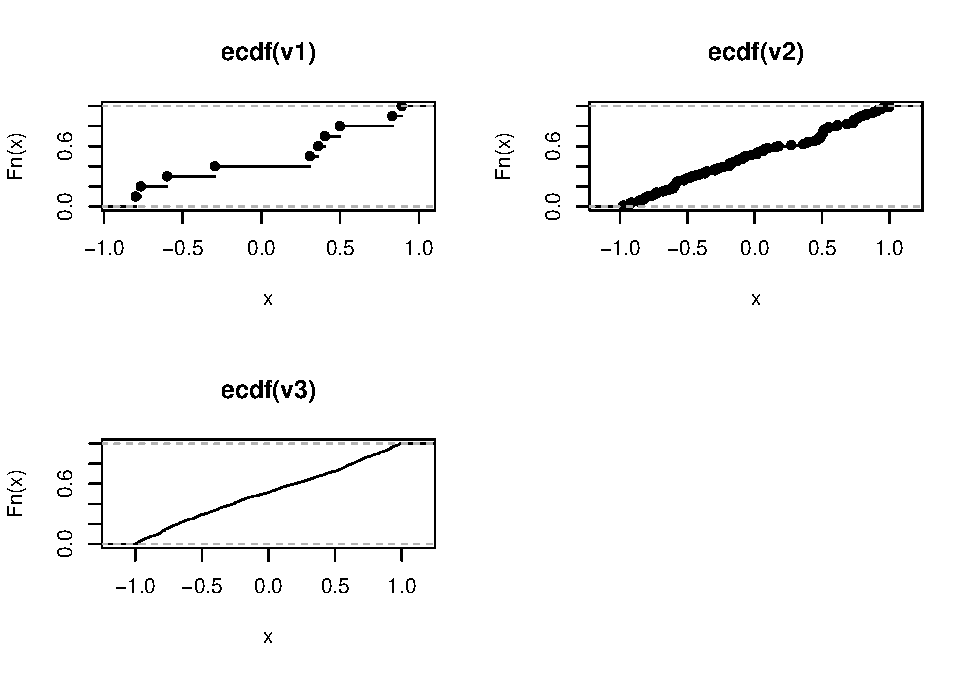
\includegraphics[width=1\linewidth,height=0.5\textheight]{R_Tricks_For_ComputationStats_files/figure-latex/unnamed-chunk-2-1}

\hypertarget{generate-data-from-exponential-distribution}{%
\subsubsection{2.3 Generate data from exponential
distribution}\label{generate-data-from-exponential-distribution}}

TODO: to summarize every prob. distribution

\begin{Shaded}
\begin{Highlighting}[]
\SpecialCharTok{\textgreater{}} \FunctionTok{set.seed}\NormalTok{(}\DecValTok{8289}\NormalTok{)}
\SpecialCharTok{\textgreater{}} \FunctionTok{par}\NormalTok{(}\AttributeTok{mfrow=}\FunctionTok{c}\NormalTok{(}\DecValTok{2}\NormalTok{,}\DecValTok{2}\NormalTok{))}
\SpecialCharTok{\textgreater{}}\NormalTok{ v1 }\OtherTok{\textless{}{-}} \FunctionTok{rexp}\NormalTok{(}\AttributeTok{n =} \DecValTok{10}\NormalTok{, }\AttributeTok{rate =}\NormalTok{ .}\DecValTok{1}\NormalTok{)}
\SpecialCharTok{\textgreater{}} \FunctionTok{plot}\NormalTok{(}\FunctionTok{ecdf}\NormalTok{(v1))}
\SpecialCharTok{\textgreater{}}\NormalTok{ v2 }\OtherTok{\textless{}{-}} \FunctionTok{rexp}\NormalTok{(}\AttributeTok{n =} \DecValTok{100}\NormalTok{, }\AttributeTok{rate =}\NormalTok{ .}\DecValTok{1}\NormalTok{)}
\SpecialCharTok{\textgreater{}} \FunctionTok{plot}\NormalTok{(}\FunctionTok{ecdf}\NormalTok{(v2))}
\SpecialCharTok{\textgreater{}}\NormalTok{ v3 }\OtherTok{\textless{}{-}} \FunctionTok{rexp}\NormalTok{(}\AttributeTok{n =} \DecValTok{1000}\NormalTok{, }\AttributeTok{rate =}\NormalTok{ .}\DecValTok{1}\NormalTok{)}
\SpecialCharTok{\textgreater{}} \FunctionTok{plot}\NormalTok{(}\FunctionTok{ecdf}\NormalTok{(v3))}
\end{Highlighting}
\end{Shaded}

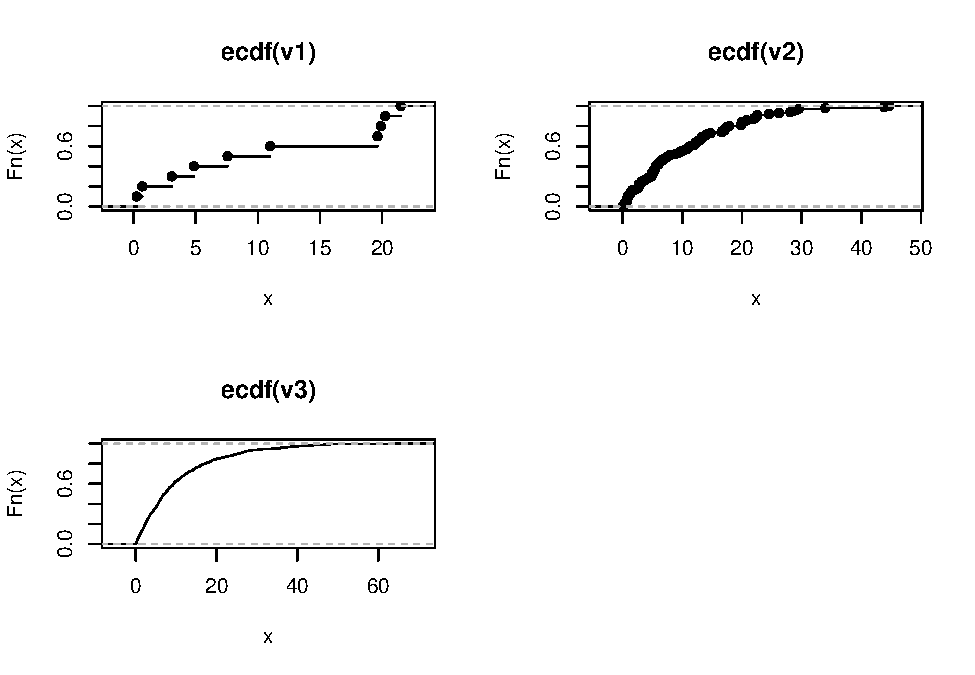
\includegraphics[width=1\linewidth,height=0.5\textheight]{R_Tricks_For_ComputationStats_files/figure-latex/unnamed-chunk-3-1}

\hypertarget{quantitle-function}{%
\subsubsection{2.4 Quantitle Function}\label{quantitle-function}}

Quantile function is actually a inverse function of CDF. That is for a
given probability, to find the greatest lower bound of value.\\
Now, let's estimate the .25 quantile for a sample from uniform
-1\textasciitilde1. Since the properties of ecdf is to give each datum a
1/n value and then to count the culmulative value of 1/n, and since this
is a uniform distribution which means each two data point shares the
same interval. Therefore the heigh change in step is 1/n

\begin{Shaded}
\begin{Highlighting}[]
\SpecialCharTok{\textgreater{}} \FunctionTok{set.seed}\NormalTok{(}\DecValTok{9832}\NormalTok{)}
\SpecialCharTok{\textgreater{}}\NormalTok{ v1 }\OtherTok{\textless{}{-}} \FunctionTok{runif}\NormalTok{(}\AttributeTok{n =} \DecValTok{10}\NormalTok{, }\AttributeTok{min=} \SpecialCharTok{{-}}\DecValTok{1}\NormalTok{, }\AttributeTok{max=} \DecValTok{1}\NormalTok{)}
\SpecialCharTok{\textgreater{}} \CommentTok{\# note ecdf is a function based on given observations}
\ErrorTok{\textgreater{}}\NormalTok{ ecdf1}\OtherTok{\textless{}{-}} \FunctionTok{ecdf}\NormalTok{(v1)}
\SpecialCharTok{\textgreater{}} \FunctionTok{plot}\NormalTok{(ecdf1)}
\SpecialCharTok{\textgreater{}} \FunctionTok{abline}\NormalTok{(}\AttributeTok{a =} \DecValTok{1}\SpecialCharTok{/}\DecValTok{2}\NormalTok{, }\AttributeTok{b =} \DecValTok{1}\SpecialCharTok{/}\DecValTok{2}\NormalTok{)}
\SpecialCharTok{\textgreater{}} \CommentTok{\# note the following is not a quantile function!!}
\ErrorTok{\textgreater{}} \FunctionTok{ecdf1}\NormalTok{(}\FloatTok{0.5}\NormalTok{)}
\NormalTok{[}\DecValTok{1}\NormalTok{] }\FloatTok{0.8}
\end{Highlighting}
\end{Shaded}

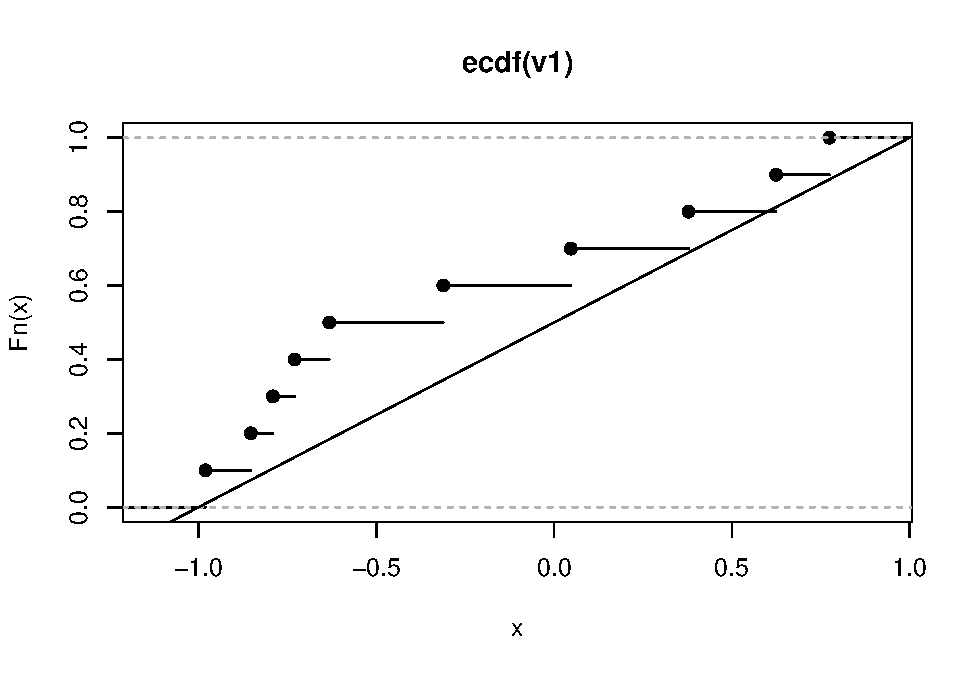
\includegraphics[width=1\linewidth,height=0.5\textheight]{R_Tricks_For_ComputationStats_files/figure-latex/unnamed-chunk-4-1}
Next, let's estimate .5 quantile via ecdf. The quantile is greatest
lower bound of set of x values for which the ecdf is greater or equal to
.5.

\begin{Shaded}
\begin{Highlighting}[]
\SpecialCharTok{\textgreater{}} \CommentTok{\# using cbind() funciton to combine tow columns of data}
\ErrorTok{\textgreater{}} \CommentTok{\# the seq is to create a set of data with certain interval}
\ErrorTok{\textgreater{}}\NormalTok{ ecdf\_tab }\OtherTok{\textless{}{-}} \FunctionTok{round}\NormalTok{(}\FunctionTok{cbind}\NormalTok{(}\FunctionTok{sort}\NormalTok{(v1), }\FunctionTok{seq}\NormalTok{(.}\DecValTok{1}\NormalTok{,}\DecValTok{1}\NormalTok{,.}\DecValTok{1}\NormalTok{)),}\DecValTok{3}\NormalTok{)}
\SpecialCharTok{\textgreater{}} \FunctionTok{colnames}\NormalTok{(ecdf\_tab) }\OtherTok{\textless{}{-}} \FunctionTok{c}\NormalTok{(}\StringTok{"x"}\NormalTok{, }\StringTok{"F(x)"}\NormalTok{)}
\SpecialCharTok{\textgreater{}}\NormalTok{ ecdf\_tab}
\NormalTok{           x }\FunctionTok{F}\NormalTok{(x)}
\NormalTok{ [}\DecValTok{1}\NormalTok{,] }\SpecialCharTok{{-}}\FloatTok{0.980}  \FloatTok{0.1}
\NormalTok{ [}\DecValTok{2}\NormalTok{,] }\SpecialCharTok{{-}}\FloatTok{0.853}  \FloatTok{0.2}
\NormalTok{ [}\DecValTok{3}\NormalTok{,] }\SpecialCharTok{{-}}\FloatTok{0.791}  \FloatTok{0.3}
\NormalTok{ [}\DecValTok{4}\NormalTok{,] }\SpecialCharTok{{-}}\FloatTok{0.730}  \FloatTok{0.4}
\NormalTok{ [}\DecValTok{5}\NormalTok{,] }\SpecialCharTok{{-}}\FloatTok{0.632}  \FloatTok{0.5}
\NormalTok{ [}\DecValTok{6}\NormalTok{,] }\SpecialCharTok{{-}}\FloatTok{0.311}  \FloatTok{0.6}
\NormalTok{ [}\DecValTok{7}\NormalTok{,]  }\FloatTok{0.047}  \FloatTok{0.7}
\NormalTok{ [}\DecValTok{8}\NormalTok{,]  }\FloatTok{0.378}  \FloatTok{0.8}
\NormalTok{ [}\DecValTok{9}\NormalTok{,]  }\FloatTok{0.625}  \FloatTok{0.9}
\NormalTok{[}\DecValTok{10}\NormalTok{,]  }\FloatTok{0.775}  \FloatTok{1.0}
\SpecialCharTok{\textgreater{}} \FunctionTok{par}\NormalTok{(}\AttributeTok{mfrow=}\FunctionTok{c}\NormalTok{(}\DecValTok{1}\NormalTok{,}\DecValTok{2}\NormalTok{))}
\SpecialCharTok{\textgreater{}} \FunctionTok{plot}\NormalTok{(ecdf\_tab)}
\SpecialCharTok{\textgreater{}} \FunctionTok{points}\NormalTok{(ecdf\_tab[}\DecValTok{5}\NormalTok{,}\DecValTok{1}\NormalTok{], ecdf\_tab[}\DecValTok{5}\NormalTok{,}\DecValTok{2}\NormalTok{], }\AttributeTok{pch =} \DecValTok{3}\NormalTok{, }\AttributeTok{col =} \DecValTok{2}\NormalTok{, }\AttributeTok{cex =} \DecValTok{2}\NormalTok{, }\AttributeTok{lwd =} \DecValTok{2}\NormalTok{)}
\SpecialCharTok{\textgreater{}} \CommentTok{\# next, lets draw a quantile function using R\textquotesingle{}s defualt}
\ErrorTok{\textgreater{}} \FunctionTok{quantile}\NormalTok{(}\AttributeTok{x =}\NormalTok{ v1, }\AttributeTok{prob =} \FloatTok{0.5}\NormalTok{)}
       \DecValTok{50}\NormalTok{\% }
\SpecialCharTok{{-}}\FloatTok{0.4718142} 
\SpecialCharTok{\textgreater{}} \FunctionTok{plot}\NormalTok{(ecdf\_tab)}
\SpecialCharTok{\textgreater{}} \FunctionTok{points}\NormalTok{(ecdf\_tab[}\DecValTok{5}\NormalTok{,}\DecValTok{1}\NormalTok{], ecdf\_tab[}\DecValTok{5}\NormalTok{,}\DecValTok{2}\NormalTok{], }\AttributeTok{pch =} \DecValTok{3}\NormalTok{, }\AttributeTok{col =} \DecValTok{2}\NormalTok{, }\AttributeTok{cex =} \DecValTok{2}\NormalTok{, }\AttributeTok{lwd =} \DecValTok{2}\NormalTok{)}
\SpecialCharTok{\textgreater{}} \FunctionTok{points}\NormalTok{(}\FunctionTok{quantile}\NormalTok{(}\AttributeTok{x =}\NormalTok{ v1, }\AttributeTok{probs =}\NormalTok{ .}\DecValTok{5}\NormalTok{), .}\DecValTok{5}\NormalTok{, }\AttributeTok{pch =} \DecValTok{4}\NormalTok{, }\AttributeTok{col =} \DecValTok{3}\NormalTok{, }\AttributeTok{cex =} \DecValTok{2}\NormalTok{, }\AttributeTok{lwd =} \DecValTok{2}\NormalTok{)}
\end{Highlighting}
\end{Shaded}

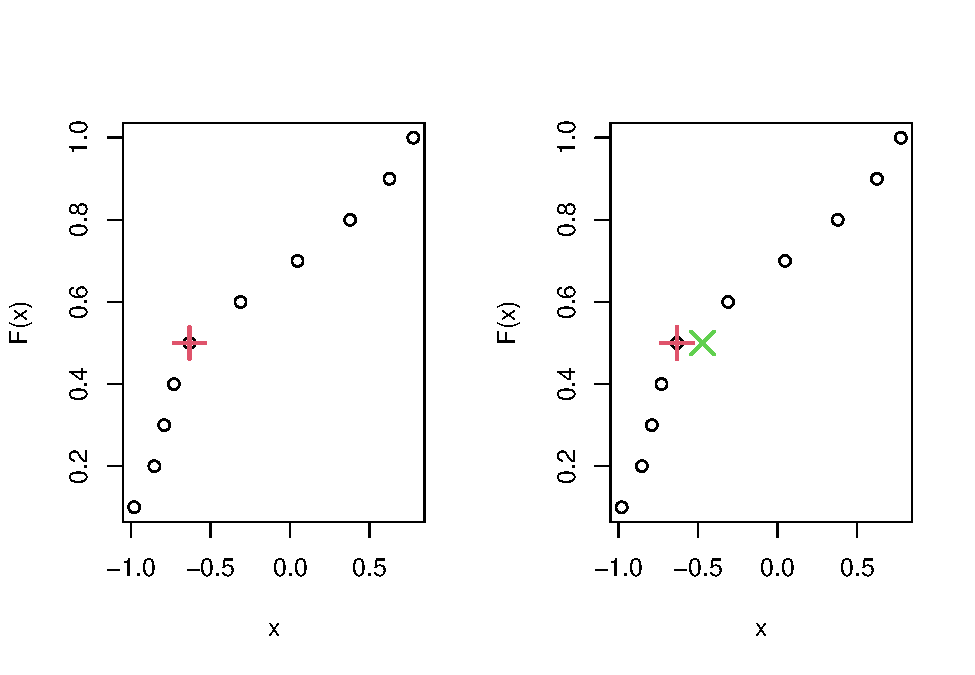
\includegraphics[width=1\linewidth,height=1\textheight]{R_Tricks_For_ComputationStats_files/figure-latex/unnamed-chunk-5-1}

By default, the \texttt{quantile()} function in R will return a
different result. Here there are n = 10 observations.R uses type = 7
which specifies that the kth order statistic is assigned cumulative
probability of (k-1)/(n-1). Furthermore, R help notes that ``All sample
quantiles are defined as weighted averages of consecutive order
statistics.''

\begin{Shaded}
\begin{Highlighting}[]
\SpecialCharTok{\textgreater{}}\NormalTok{ type7\_tab }\OtherTok{\textless{}{-}} \FunctionTok{round}\NormalTok{(}\FunctionTok{cbind}\NormalTok{(}\FunctionTok{sort}\NormalTok{(v1), }\FunctionTok{seq}\NormalTok{(}\DecValTok{0}\NormalTok{, }\DecValTok{1}\NormalTok{, }\DecValTok{1}\SpecialCharTok{/}\DecValTok{9}\NormalTok{)), }\DecValTok{3}\NormalTok{)}
\SpecialCharTok{\textgreater{}} \FunctionTok{colnames}\NormalTok{(type7\_tab) }\OtherTok{\textless{}{-}} \FunctionTok{c}\NormalTok{(}\StringTok{"x"}\NormalTok{, }\StringTok{"F(x)"}\NormalTok{)}
\SpecialCharTok{\textgreater{}}\NormalTok{ type7\_tab}
\NormalTok{           x  }\FunctionTok{F}\NormalTok{(x)}
\NormalTok{ [}\DecValTok{1}\NormalTok{,] }\SpecialCharTok{{-}}\FloatTok{0.980} \FloatTok{0.000}
\NormalTok{ [}\DecValTok{2}\NormalTok{,] }\SpecialCharTok{{-}}\FloatTok{0.853} \FloatTok{0.111}
\NormalTok{ [}\DecValTok{3}\NormalTok{,] }\SpecialCharTok{{-}}\FloatTok{0.791} \FloatTok{0.222}
\NormalTok{ [}\DecValTok{4}\NormalTok{,] }\SpecialCharTok{{-}}\FloatTok{0.730} \FloatTok{0.333}
\NormalTok{ [}\DecValTok{5}\NormalTok{,] }\SpecialCharTok{{-}}\FloatTok{0.632} \FloatTok{0.444}
\NormalTok{ [}\DecValTok{6}\NormalTok{,] }\SpecialCharTok{{-}}\FloatTok{0.311} \FloatTok{0.556}
\NormalTok{ [}\DecValTok{7}\NormalTok{,]  }\FloatTok{0.047} \FloatTok{0.667}
\NormalTok{ [}\DecValTok{8}\NormalTok{,]  }\FloatTok{0.378} \FloatTok{0.778}
\NormalTok{ [}\DecValTok{9}\NormalTok{,]  }\FloatTok{0.625} \FloatTok{0.889}
\NormalTok{[}\DecValTok{10}\NormalTok{,]  }\FloatTok{0.775} \FloatTok{1.000}
\SpecialCharTok{\textgreater{}} \CommentTok{\# Weighted avg of consecutive order statistics.}
\ErrorTok{\textgreater{}} \FunctionTok{mean}\NormalTok{(type7\_tab[}\DecValTok{5}\SpecialCharTok{:}\DecValTok{6}\NormalTok{,}\DecValTok{1}\NormalTok{])}
\NormalTok{[}\DecValTok{1}\NormalTok{] }\SpecialCharTok{{-}}\FloatTok{0.4715}
\SpecialCharTok{\textgreater{}} \CommentTok{\# the value is same to the quantile function}
\end{Highlighting}
\end{Shaded}

\hypertarget{multivariate-normal-distribution}{%
\subsubsection{2.5 Multivariate Normal
Distribution}\label{multivariate-normal-distribution}}

\begin{Shaded}
\begin{Highlighting}[]
\SpecialCharTok{\textgreater{}} \CommentTok{\# Generate multivariate normal}
\ErrorTok{\textgreater{}}\NormalTok{ mvn\_gen }\OtherTok{\textless{}{-}} \ControlFlowTok{function}\NormalTok{(n, mu, sigma, }\AttributeTok{factorization =} \StringTok{"Cholesky"}\NormalTok{) \{}
\SpecialCharTok{+}   \CommentTok{\# Generate a sample of size n from multivariate normal with}
\SpecialCharTok{+}   \CommentTok{\# mean vector mu and covariance matrix sigma.}
\SpecialCharTok{+}   \CommentTok{\# Argument factorization can be either "Cholesky" or "Spectral".}
\SpecialCharTok{+}\NormalTok{   d }\OtherTok{\textless{}{-}} \FunctionTok{length}\NormalTok{(mu)}
\SpecialCharTok{+}\NormalTok{   Z }\OtherTok{\textless{}{-}} \FunctionTok{matrix}\NormalTok{(}\FunctionTok{rnorm}\NormalTok{(n}\SpecialCharTok{*}\NormalTok{d), }\AttributeTok{nrow =}\NormalTok{ n, }\AttributeTok{ncol =}\NormalTok{ d)}
\SpecialCharTok{+}   \ControlFlowTok{if}\NormalTok{(factorization }\SpecialCharTok{==} \StringTok{"Cholesky"}\NormalTok{) \{ Q }\OtherTok{\textless{}{-}} \FunctionTok{chol}\NormalTok{(sigma) \} }\ControlFlowTok{else}\NormalTok{ \{}
\SpecialCharTok{+}     \ControlFlowTok{if}\NormalTok{(factorization }\SpecialCharTok{==} \StringTok{"Spectral"}\NormalTok{) \{}
\SpecialCharTok{+}\NormalTok{       ev }\OtherTok{\textless{}{-}} \FunctionTok{eigen}\NormalTok{(sigma)}
\SpecialCharTok{+}\NormalTok{       lambda }\OtherTok{\textless{}{-}}\NormalTok{ ev}\SpecialCharTok{$}\NormalTok{values}
\SpecialCharTok{+}\NormalTok{       P }\OtherTok{\textless{}{-}}\NormalTok{ ev}\SpecialCharTok{$}\NormalTok{vectors}
\SpecialCharTok{+}\NormalTok{       Q }\OtherTok{\textless{}{-}}\NormalTok{ P }\SpecialCharTok{\%*\%} \FunctionTok{diag}\NormalTok{(}\FunctionTok{sqrt}\NormalTok{(lambda)) }\SpecialCharTok{\%*\%} \FunctionTok{t}\NormalTok{(P) \} }\ControlFlowTok{else}\NormalTok{ \{}
\SpecialCharTok{+}         \FunctionTok{stop}\NormalTok{(}\StringTok{"Arg factorization must be \textquotesingle{}Cholesky\textquotesingle{} or \textquotesingle{}Spectral\textquotesingle{}."}\NormalTok{)}
\SpecialCharTok{+}\NormalTok{       \} \}}
\SpecialCharTok{+}\NormalTok{   mu }\OtherTok{\textless{}{-}} \FunctionTok{matrix}\NormalTok{(mu, }\AttributeTok{nrow =}\NormalTok{ d, }\AttributeTok{ncol =} \DecValTok{1}\NormalTok{)}
\SpecialCharTok{+}\NormalTok{   J }\OtherTok{=} \FunctionTok{matrix}\NormalTok{(}\DecValTok{1}\NormalTok{, }\AttributeTok{nrow =}\NormalTok{ n, }\AttributeTok{ncol =} \DecValTok{1}\NormalTok{)}
\SpecialCharTok{+}\NormalTok{   X }\OtherTok{\textless{}{-}}\NormalTok{ Z }\SpecialCharTok{\%*\%}\NormalTok{ Q }\SpecialCharTok{+}\NormalTok{ J }\SpecialCharTok{\%*\%} \FunctionTok{t}\NormalTok{(mu)}
\SpecialCharTok{+}   \FunctionTok{return}\NormalTok{(}\FunctionTok{data.frame}\NormalTok{(X))}
\SpecialCharTok{+}\NormalTok{ \}}
\SpecialCharTok{\textgreater{}} 
\ErrorTok{\textgreater{}}\NormalTok{ sig }\OtherTok{\textless{}{-}} \FunctionTok{matrix}\NormalTok{(}\FunctionTok{c}\NormalTok{(}\DecValTok{1}\NormalTok{, .}\DecValTok{5}\NormalTok{, .}\DecValTok{8}\NormalTok{, .}\DecValTok{5}\NormalTok{, }\DecValTok{1}\NormalTok{, }\DecValTok{0}\NormalTok{, .}\DecValTok{8}\NormalTok{, }\DecValTok{0}\NormalTok{, }\DecValTok{1}\NormalTok{), }\DecValTok{3}\NormalTok{, }\DecValTok{3}\NormalTok{, }\AttributeTok{byrow =} \ConstantTok{TRUE}\NormalTok{)}
\SpecialCharTok{\textgreater{}} 
\ErrorTok{\textgreater{}} \FunctionTok{set.seed}\NormalTok{(}\DecValTok{2381}\NormalTok{)}
\SpecialCharTok{\textgreater{}}\NormalTok{ mv1 }\OtherTok{\textless{}{-}} \FunctionTok{mvn\_gen}\NormalTok{(}\AttributeTok{n =} \DecValTok{1000}\NormalTok{, }\AttributeTok{mu =} \FunctionTok{c}\NormalTok{(}\DecValTok{0}\NormalTok{, }\DecValTok{1}\NormalTok{, }\DecValTok{4}\NormalTok{), }\AttributeTok{sigma =}\NormalTok{ sig, }\AttributeTok{factorization =} \StringTok{"Cholesky"}\NormalTok{)}
\SpecialCharTok{\textgreater{}} \FunctionTok{plot}\NormalTok{(mv1)}
\SpecialCharTok{\textgreater{}}\NormalTok{ mv2 }\OtherTok{\textless{}{-}} \FunctionTok{mvn\_gen}\NormalTok{(}\AttributeTok{n =} \DecValTok{1000}\NormalTok{, }\AttributeTok{mu =} \FunctionTok{c}\NormalTok{(}\DecValTok{0}\NormalTok{, }\DecValTok{1}\NormalTok{, }\DecValTok{4}\NormalTok{), }\AttributeTok{sigma =}\NormalTok{ sig, }\AttributeTok{factorization =} \StringTok{"Spectral"}\NormalTok{)}
\SpecialCharTok{\textgreater{}} \FunctionTok{plot}\NormalTok{(mv2)}
\end{Highlighting}
\end{Shaded}

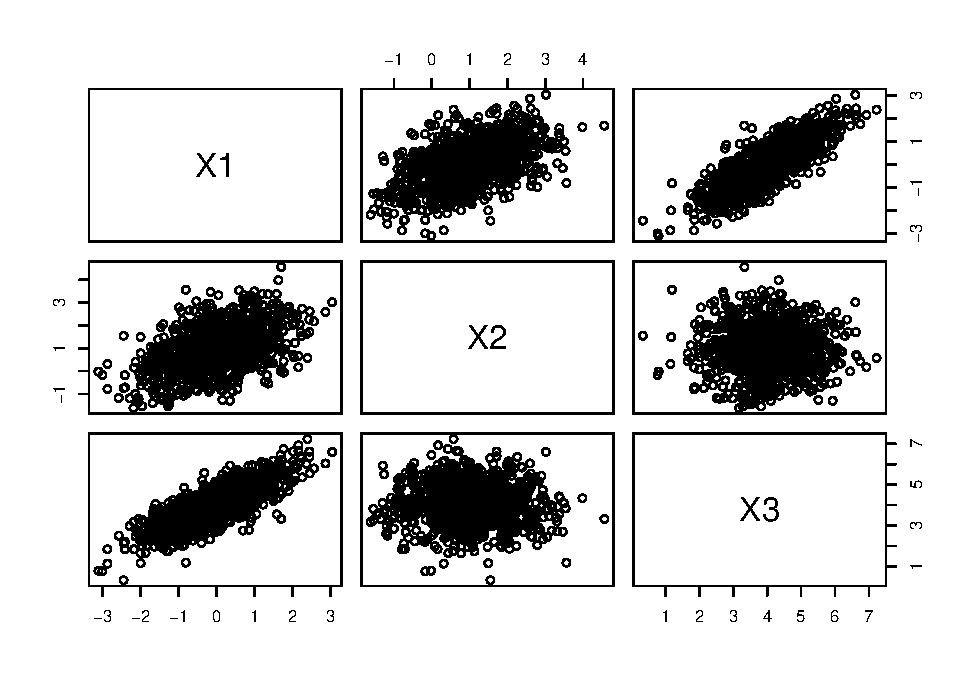
\includegraphics[width=0.5\linewidth,height=0.5\textheight]{R_Tricks_For_ComputationStats_files/figure-latex/unnamed-chunk-7-1}
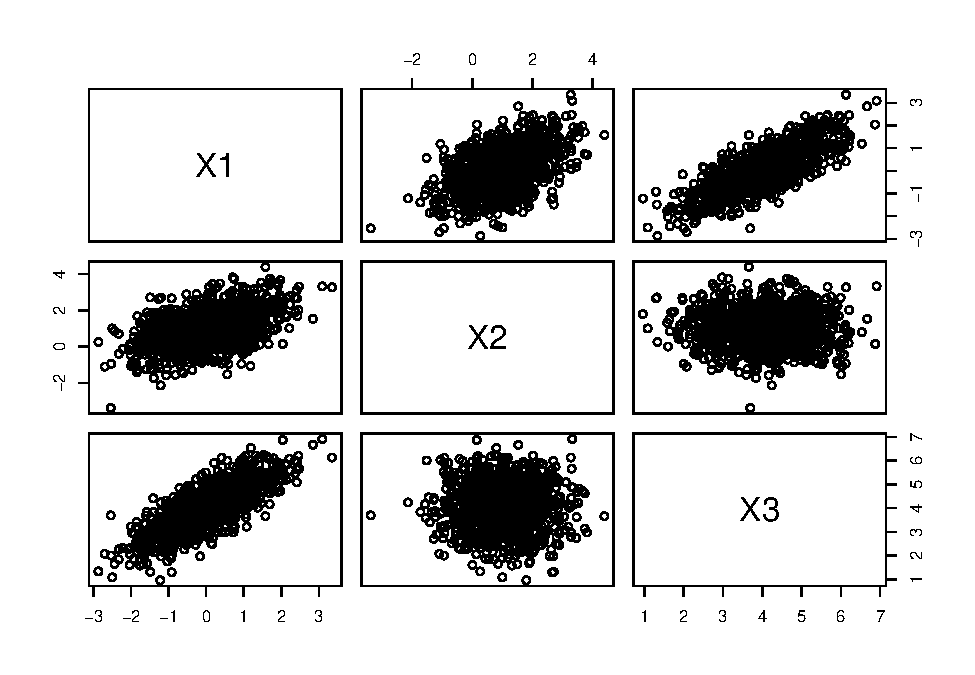
\includegraphics[width=0.5\linewidth,height=0.5\textheight]{R_Tricks_For_ComputationStats_files/figure-latex/unnamed-chunk-7-2}

\end{document}
